\section{Adaptive Wildlife Encounter protocol}
\label{sectionprotocol}

In this section, we present our encounter registration protocol.
The pseudo-code of the protocol is given in Algorithm~\ref{DA} and Algorithm~\ref{CA}.

The protocol consists of two stages: detecting stage and connecting stage. 
\begin{itemize}
    \item \textbf{Stage 1: detecting stage.} In this stage, an agent attempts to
    detect whether there are nearby peers, regardless of who they are. 
    \item \textbf{Stage 2: connecting stage} In this stage, an agent attempts to 
    identify the nearby peer(s) and record their IDs to its log.
\end{itemize}

Initially, each agent starts from the detecting stage. 
In the detecting stage, an agent turns its radio to the $sleep$ state most of the time,
and switches to $transmit$ state or $listen$ state at intervals.
In the connecting stage, agents only switch between $transmit$ state 
and $listen$ state.

The key idea of {\pName} is that, any single agent keeps in detecting 
stage to reduce ineffective energy consumption. When encounter happens, 
it detects the existence of nearby peers and turns to the connecting stage 
to identify those peers (or a peer) as fast as possible, and record the encounter process to its log. 
when the encounter process is determined to be finished in the connecting stage, 
the agent turns back to the detecting stage.

\begin{remark}
    In {\pName}, there is no need to synchronize the stage between agents and
    {\pName} still works when encounter peers are in different stage, e.g., an agent in detecting 
    stage comes into a stable clique in connecting stage. 
    The proof of correctness will be presented 
    in section~\ref{proof}. 
\end{remark}

In the following, we describe the operations of these two stages in detail. 

\subsection{Detecting stage}

In the detecting stage,  
energy efficiency is achieved by the duty cycle mechanism, 
e.g., denote the predefined duty cycle for 
all the agents is $\theta$, the tag radio of each agent will work
$\theta T_0$ slots in every period of $T_0$ slots. 

However, it is very ineffective
when two agents encounter and one is in $sleep$ state while the other is transmitting
or listening. 
To technically achieve synchronizing the time that agents turn on the radio without extra cost,
we introduce the technique of Relax Difference Set (RDS)~\cite{luk1997two}.
We use the RDS technique to guarantee that every encounter pair 
of agents turn on the radio in the same slot at least once in each round $T_0$.

RDS is an efficient tool to construct cyclic quorum systems~\cite{Peleg1995The}. 
The definition is:
\begin{definition}
A set $R=\{a_1,a_2,...,a_k\} \subseteq Z_T$ (the set of all non-negative integers less than $T$)
is called a RDS if for every $d \neq 0$ (mod $T$),
there exists at least one ordered pair $(a_i,a_j)$ such that $a_i - a_j \equiv d$ (mod $T$), 
where $a_i,a_j \in D$.
\end{definition}

\begin{figure}[h]
    \centering
    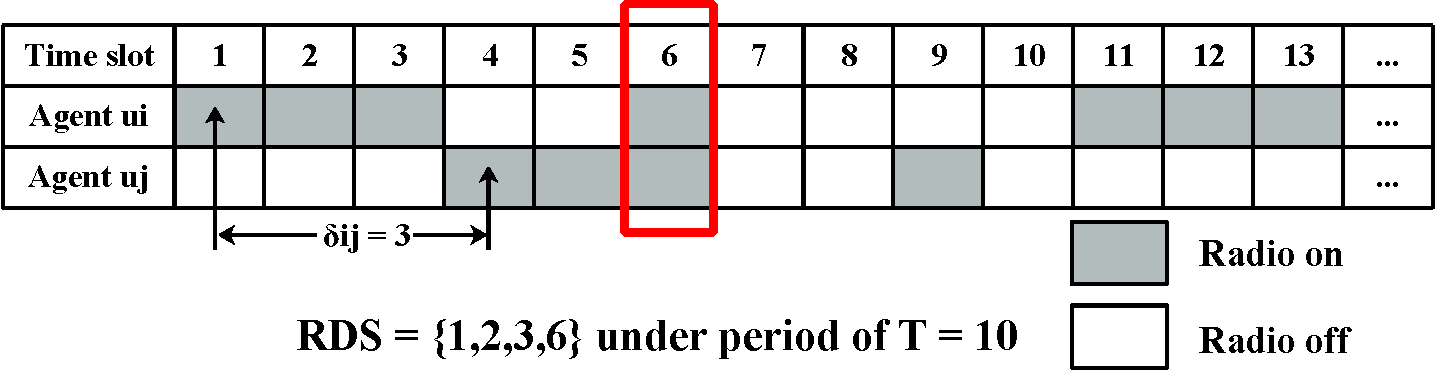
\includegraphics[width=3.5in]{figures/RDS}
    \caption{A example of how RDS works to help synchronization. Consider a period
    of $ten$ slots and the time drift between two agents $u_i$ and 
    $u_j$ is $3$. There exists an ordered pair $(6,3)$ in the constructed RDS such that $6 - 3 \equiv 3$ (mod $10$). Thus 
    they will determinately turn on the radio at the same slot in every period $T$, 
    which is the $6^{th}$ slot in a period of $u_i$ and the $3^{th}$ slot in that of $u_j$ respectively.}
    \label{exampleRDS}
\end{figure}

We now give an example to explain how RDS works to help synchronization.
Suppose the duty cycle is set as $0.4$, i.e., there are $4$ active slots 
in every $10$ slots. It is easy to show that $R=\{1,2,3,6\}$ is a RDS
under $Z_{10}$:
\begin{align*}
    &2 - 1 = 1,\quad 3 - 1 = 2,\quad 6 - 3 = 3,\quad 6 - 2 = 4, \\
    &6 - 1 = 5,\quad {2 - 6 = 6}~{(mod~10)},\quad \dots,\quad \dots, 
\end{align*}
In every period of ten slots, for any $i = \{0,1,\dots,9\}$, if $i \in R$, then
the agent turns on its radio in the $i^{th}$ slot in this period; otherwise it turns off the 
radio to the $sleep$ state. An example is depicted in Figure~\ref{exampleRDS}. 



\begin{algorithm}[!h]
    \caption{RDS Construction Algorithm}
    \label{RDS}
    \begin{algorithmic}[1]
    \STATE $R :=\emptyset$; $\lambda :=\lceil \sqrt{N}  \rceil$,
    $\mu :=\lceil \frac{\lceil \sqrt{N} \rceil}{2} \rceil$;\label{RDSline1}
    \FOR{$i = 1 :\lambda$}
        \STATE $R :=R \cup i$; \label{RDSline2}
    \ENDFOR
    \FOR{$j = 1 :\mu$}
        \STATE $R :=R \cup (1 + j * \lambda )$; \label{RDSline3}
    \ENDFOR
    \end{algorithmic}
\end{algorithm}

It has been proved that any RDS must have cardinality $|R| \geq \sqrt{N}$\cite{luk1997two}.
We present a linear algorithm to construct a RDS with 
cardinality $\lceil \frac{3\sqrt{T_0}}{2}  \rceil$ under $Z_{T_0}$ in Alg. \ref{RDS}.

We show the correctness of the construction formally.
%The correctness proof of the construction
\begin{lemma}
\label{RDS1}
Set $R = \{r_0, r_1, ..., r_{\lambda + \mu - 1}\}$ constructed in Alg. \ref{RDS} is a RDS,
where $|R| = \lambda + \mu = \lceil \sqrt{T_0}  \rceil + \lceil \frac{\lceil \sqrt{T_0} \rceil}{2} \rceil
\approx \lceil \frac{3\sqrt{T_0}}{2}  \rceil$.
\end{lemma}
\begin{IEEEproof}
Obviously, if there exists one ordered pair $(a_i,a_j)$ satisfying  $a_i - a_j \equiv d$ (mod $T_0$),
an opposing pair $(a_j,a_i)$ exists such that
$a_j - a_i \equiv (T_0-d)$ (mod $T_0$). Thus we only need to find
at least one ordered pair $(a_i,a_j)$ for each $d \in [1, \lfloor T_0/2 \rfloor]$.

In the construction, $\lambda$ in Line \ref{RDSline1} is the smallest integer satisfying
$\lambda^2 \geq T_0$. Every $d$ in range $[1, \lfloor T_0/2 \rfloor]$
can be represented as: $ d = 1 + j \times \lambda - i$, where $1 \leq j \leq \mu,
1 \leq i \leq \lambda$. Thus, there exists $a_j = 1 + j \times \lambda$
from Line. \ref{RDSline2} and $a_i = i$ from Line. \ref{RDSline3}
satisfying  $a_j - a_i \equiv d$. Then, the lemma can be derived.
\end{IEEEproof}

\begin{algorithm}[!h]
    \caption{Detecting Algorithm}
    \label{DA}
    \begin{algorithmic}[1]
    \STATE $T_0 := \lceil \frac{9}{4\theta^{2}} \rceil$; $\omega_0 :=\frac{1}{2}$; $t := 0$;
    \STATE Invoke Alg.~\ref{RDS} to construct $R = \{r_0, r_1, ...,r_{\lceil 
    \frac{3\sqrt{T_0}}{2}  \rceil}\}$ under $Z_{T_0}$;
    \WHILE {$True$}
        \IF{$(t + 1) \in R$}  \label{On}
            \STATE \textbf{\emph{In the first sub-slot:}}
            \STATE Transmit a beacon with probability $\omega_0$
            and listen with probability $1-\omega_0$;
            \STATE \textbf{\emph{In the second sub-slot:}}
            \IF{the agent is in $listen$ state in the first sub-slot}
                \IF{detects~energy~(a~beacon~or~a~collision~by~multiple~beacons)~in~the~first~sub-slot}
                    \STATE Transmit a beacon and turn to the \textbf{connecting stage};
                \ENDIF
            \ELSIF{detects~energy~(a~beacon~or~a~collision~by~multiple~beacons)~in~this~sub-slot}
                \STATE Turn to the \textbf{connecting stage};
            \ENDIF
        \ELSE
                \STATE $Sleep$ in the whole slot;
        \ENDIF
        \STATE $t := (t + 1) \% T_0$;
    \ENDWHILE
    \end{algorithmic}
\end{algorithm}

Based on the RDS, we present the operations in the detecting stage, as depicted in Alg.~\ref{DA}.
Agents turn on and off the radio according to the RDS sequence.
Consider a slot the radio is on, and then the slot is divided into two sub-slots. In the first sub-slot
an agent transmits a beacon with probability $\omega_0$ and listens with probability $(1-\omega_0)$.
In the second sub-slot: 
\begin{itemize}
    \item[1)] The agent is in $listen$ state in the first sub-slot:
    \begin{itemize}
    \item if the agent detects a beacon (or beacons) in the first sub-slot, it 
    transmits a beacon (a bit is OK) as an acknowledgement 
    on the channel in the second sub-slot and turn to the 
    connecting stage; otherwise it does nothing. 
    \end{itemize}
    \item[2)] The agent is in $transmit$ state in the first sub-slot:
    \begin{itemize}
    \item if the agent detects a beacon (or beacons) in this sub-slot,
    it turns to the connecting stage; otherwise it does nothing.
    \end{itemize}
\end{itemize}

As discussed before, the aim of this stage is to detect nearby peer(s) as fast as possible 
(if exists), and either successful transmission or detecting busy on the channel activates the agent
to switch to the connecting stage. %Hence we fix the transmitting probability as $\omega_0 = \frac{1}{2}$. 

% \begin{remark}
%     Though $\omega_0 = \frac{1}{2}$ is not the optimal probability in multi-agent encounter cases, 
%     the probability that an agent detects a peer in a slot grows as the number of agents
%     increases. This is because a new agent will not interrupt but help other agents to detect peers
%     if it is in $transmit$ state in a slot.
% \end{remark}

\subsection{Connecting stage}

In the connecting stage, agents attempt to identify the nearby 
peers and record the encounter process~(messages containing peers' IDs) to its local log.
A successful identification happens only if the agent is listening
and only one peer is transmitting. 

\begin{algorithm}[ht]
    \caption{Connecting Algorithm}
    \label{CA}
    \begin{algorithmic}[1]
    \STATE $t := 0$; $\omega_t := \zeta$; 
    \WHILE {$True$}
        \STATE \textbf{\emph{In the first sub-slot:}}
        \STATE Transmit a message containing ID with probability $\omega_t$
        and listen with probability $1-\omega_t$;
        \STATE \textbf{\emph{In the second sub-slot:}}
        \IF{the agent is in $listen$ state in the first sub-slot}
            \IF{reveive a message successfully}
                \STATE Record the source ID and transmit a beacon;
                \STATE Set $\omega_{t+1} := \frac{\omega_t}{(1+\epsilon)}$;
            \ELSIF{channel is idle}
                \STATE Set $\omega_{t+1} := min\{(1+\epsilon)\cdot\omega_t, \zeta\}$;
            \ELSE
                \STATE Set $\omega_{t+1} := \frac{\omega_t}{(1+\epsilon)}$; %$\backslash\backslash$ the channel is busy
            \ENDIF
        \ELSE
            \IF{detect beacons in this sub-slot}
                \STATE $\omega_{t+1} := 0$;
            \ELSE
                \STATE Set $\omega_{t+1} := \frac{\omega_t}{(1+\epsilon)}$;
            \ENDIF
        \ENDIF
        \STATE $t := (t + 1)$;
        \IF{$t == \hat{T}$}
            \IF{no peer is found in this round}
                \STATE Turn to the \textbf{detecting stage}; \label{backDS}
            \ELSE
                \STATE $t := 0$; $\omega_t := \zeta$;
            \ENDIF
        \ENDIF
    \ENDWHILE
    \end{algorithmic}
\end{algorithm}



The collision detection (CD) mechanism is incorporated in this stage 
to increase of efficiency. This mechanism enables the listening agent 
to notify the transmitting peers of the transmission outcomes, 
and thus they take measures to reduce the collisions if not successful.

In this stage, every $\hat{T}$ slots consists of a round. Each 
agent repeats the operations in Alg.~\ref{CA} round by round and 
it turns to the connecting stage when it cannot find any peer in a complete round, 
as the operation in Line~\ref{backDS}.

As discussed in section~\ref{sectionmodel}, $\hat{T}$ is relatively short in 
real world, thus the communication connectivity stays stable in a round. 
However, due to the dynamic movements of agents, the communication connectivity
may change from round to round, so all the parameters will be 
initialized at the beginning of each round and adaptively adjusted later 
according to the transmission outcome.

Each slot is divided into two sub-slots.
Agents execute transmission or reception in the first sub-slot, 
and in the second sub-slot take actions responding to the outcome of the previous sub-slot
(success/fail to transmit/receive a message).
% (if receive a message 
% successfully in the first sub-slot). %The algorithm in detecting stage is formulated as Alg.~\ref{CA}.

Since the number of the nearby peers is unknown to each agent, 
the transmitting probability is initially set as $\zeta$, which is a pre-defined constant.

In the first sub-slot of each slot $t$, an agent transmits a message containing ID 
with probability $\omega_t$ and listen with probability $(1 - \omega_t)$. 
In the second sub-slot: 
\begin{itemize}
    \item[1)] The agent is in $listen$ state in the first sub-slot:
    \begin{itemize}
    \item if the agent receives a message successfully, it 
    decodes and records the source ID in the message, and
    transmits a beacon (a bit is OK) as an acknowledgement 
    on the channel in the second sub-slot. 
    \item if the channel is idle, this means there is a chance to 
    transmit successfully and it multiplies its transmitting 
    probability by a factor $(1+\epsilon)$ (no larger than the pre-defined constant $\zeta$).
    \item if the agent detects collisions, it divides its transmission 
    probability by a factor ${(1+\epsilon)}$. 
    \end{itemize}
    \item[2)] The agent is in $transmit$ state in the first sub-slot:
    \begin{itemize}
    \item if the agent detects beacons in this sub-slot,
    this means its previous message has been successfully received by its nearby
    peers, and it keeps listening in all the rest first sub-slots of this round,
    which is called \emph{quiet} state.
    \item if the agent detects nothing in this sub-slot, it means its previous message
    failed to propagate due to simultaneous transmissions. Thus it divides its transmitting 
    probability by a factor ${(1+\epsilon)}$. 
    \end{itemize}
\end{itemize}

Factor ${(1+\epsilon)}$ is a pre-defined constant to adjust the transmitting probability adaptively.
For simplify, we set $(1+\epsilon) := 2$ for analysis in the next section.
In the end of a complete round, if there is no peer detected in this whole round, 
which indicates the encounter process is finished, the agent turns to the detecting stage .

\subsection{Analysis of stage switch}
\label{proof}

When an encounter happens, an agent in detecting stage will switch to connecting stage very soon. 
We derive this conclusion from the following three lemmas.

\begin{lemma}
    \label{RDS}
    Consider any two agents $u_i$ and $u_j$ in detecting stage.
    In each period $T_0$, they will turn on the radio in the same slot at least once.
\end{lemma}
\begin{IEEEproof}
Assume the time drift between $u_i$ and $u_j$ is $\delta_{ij}$ (mod $T_0$).
In the RDS constructed under $T_0$, there exists at least one ordered pair $(a_i,a_j)$ such that $a_i - a_j \equiv \delta_{ij}$ (mod $T_0$).
Thus the $a_i^{th}$ slot in a period of $u_i$ is exactly the $a_j^{th}$ slot in a period of $a_j^{th}$ and both of them
turn on the radio in this slot according to Alg.~\ref{DA} Line~\ref{On}, which completes the proof.
\end{IEEEproof}

\begin{lemma}
    \label{dtoc}
    Consider $k$ agents all in the detecting stage at the beginning, 
    an agent in detecting stage will turn to the connecting stage in 
    $O(\theta^{-2})$ slots with high probability.
\end{lemma}
\begin{IEEEproof}
    By Lemma~\ref{RDS}, an agent can turn on the radio in the same 
    slot with any other peer at least once during a period of $T_0$.
    The probability it detects a peer in a period of $T_0$ is at least
    $Pr \geq 1 - \frac{1}{2^{k-1}}$.
    Hence given a small enough constant $\eta$,  
    it holds with high probability that an agent will turn to connecting stage in 
    $\frac{\ln\eta}{\ln\frac{1}{2^{k-1}}}$ periods, which is 
    $\frac{\ln\eta}{\ln\frac{1}{2^{k-1}}} \lceil \frac{9}{4\theta^{2}} \rceil$ slots
    in total.    
\end{IEEEproof}
\vspace{0.1in}
\begin{lemma}
    \label{case}
    An agent turns to the connecting stage will increase the probability that other
    peers in the detecting stage to detect peers.
\end{lemma}
\begin{IEEEproof}
    An agent in the detecting stage will transmit or listen in every first sub-slot 
    which can help peers to detect it,
    while it only turns on the radio a fraction of time in the detecting stage.
\end{IEEEproof}
   
According to Lemma~\ref{dtoc} and \ref{case}, every agent will turn to the connecting stage in 
$O(\theta^{-2})$ slots with high probability. 